\item [17]

A \textit{T flip-flop} ("toggle" flip-flop) is a synchronous device with the following specification:

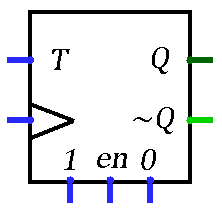
\includegraphics[height=2.0cm]{images/T-FF.png}

\begin{tabular}{c | l}
$T$ & function \\
\hline
0 & $Q^{+}=Q$ \\
1 & $Q^{+}=\sim Q$ \\

\end{tabular}

In other words, the state of the flip-flop remains unchanged if $T=0$ during a rising clock edge, and the state of the flip-flop is negated (toggled) if $T=1$ during a rising clock edge. The inputs $1$, $en$, and $0$ are asynchronous set/enable/reset -- for the most part, $en$ can be connected to constant-1, and set/reset can be connected to constant-0 during ordinary usage.

\begin{question}{a.}[4]

\item[3] Logisim provides a T flip-flop in the "Memory" library. For this question, you will use a single J-K flip-flop and logic gates to construct your own T flip-flop.

Complete the characteristic/excitation table below to determine the required inputs to the J-K flip-flop, and write your input equations for $J$ and $K$.
\\
{\color{NavyBlue}
\begin{tabular}{c c | c | c c}
$Q$ & $T$ & $Q^{+}$ & $J$ & $K$ \\
\hline
0 & 0 & 0 & 0  & 0  \\
0 & 1 & 1 & 1  & 1  \\
1 & 0 & 1 & 0  & 0  \\
1 & 1 & 0 & 1  & 1  \\
\end{tabular}

$J = T $

$K = T $
}

\item[2] \label{q-tff} Based on your input equations determined earlier, in Logisim use a J-K flip-flop and logic gates to construct a circuit that has the required behaviour of a T flip-flop. Show your circuit diagram here. Adjust your device appearance so it matches the illustration given at the top of this page.

\\
\\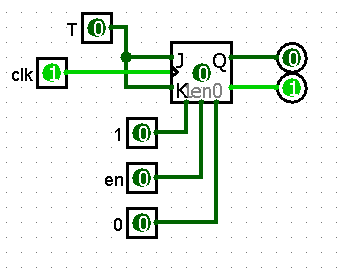
\includegraphics{q6-1-1.PNG}
\\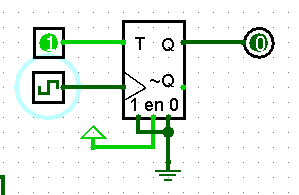
\includegraphics{q6-1-2.PNG}
\\
The Program Counter (PC) is a critical component of many past and modern CPUs, whose responsibility is to hold the address of the next program instruction to be retrieved from memory. In a typical program, instructions are executed sequentially, and so subsequent instructions are stored in consecutive addresses in memory, and the PC simply needs to increment its stored value to correctly reference the next instruction. However, many programs include branching conditionals and loops, where the next instruction to execute is found at a memory address which is not immediately following the current address stored in PC. Thus, the PC must have the ability to be loaded with an arbitrary address so that the instruction beginning the conditional branch or loop can be executed next. In summary, the PC can be described as an incrementing counter, with parallel load and clear. The full functionality will be described in a later part of this assignment, but we will achieve all the required functionality by first building simpler components which satisfy partial functionality.

We will begin by designing components to achieve the parallel load functionality. A 1-bit load register has the following specification:

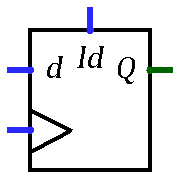
\includegraphics[height=2.0cm]{images/load-1.png}

\begin{tabular}{c | l}
$ld$ & function \\
\hline
0 & $Q^{+}=Q$ (no change) \\
1 & $Q^{+}=d$ \\
\end{tabular}

Specifically, when $ld=0$, the device remains unchanged, and when $ld=1$, the value observed on the input $d$ is loaded into the device.

\item[2] You will use the T flip-flop constructed in part \ref{q-tff} to construct the 1-bit load register.

Complete the characteristic/excitation table below to determine the required inputs to the T flip-flop, and write your input equations for $T$.

{\color{NavyBlue}
\begin{tabular}{c c c | c | c}
$Q$ & $ld$ & $d$ & $Q^{+}$ & $T$ \\
\hline
0 & 0 & 0 & 0  & 0  \\
0 & 0 & 1 & 0  & 0  \\
0 & 1 & 0 & 0  & 0  \\
0 & 1 & 1 & 1  & 1  \\
\hline
1 & 0 & 0 & 1  & 0  \\
1 & 0 & 1 & 1  & 0  \\
1 & 1 & 0 & 0  & 1  \\
1 & 1 & 1 & 1  & 0  \\
\end{tabular}

$T = ld \land (Q (+) d)$
}

\item[2] \label{q-ld1} Based on your input equation determined above, in Logisim use your T flip-flop and logic gates to construct a circuit that has the required behaviour of the 1-bit load register. It is recommended to connect power and ground devices to the asynchronous set/enable/reset inputs appropriately. Show your circuit diagram here. Adjust your device appearance so it matches the illustration given above.

\\
\\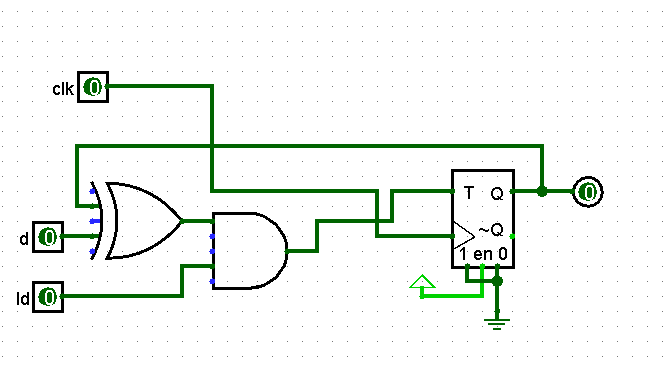
\includegraphics{q6-2-1.PNG}
\\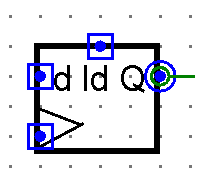
\includegraphics{q6-2-2.PNG}
\\

The 1-bit load register can be connected in parallel to construct larger parallel load registers. A 4-bit parallel load register is described below:

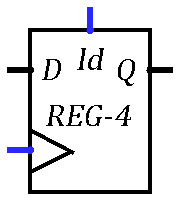
\includegraphics[height=2.0cm]{images/reg-4.png}

\begin{tabular}{c | l}
$ld$ & function \\
\hline
0 & No change \\
1 & $Q \leftarrow D$ \\
\end{tabular}

The behaviour is the same as the 1-bit load register, with the understanding that $Q$ and $D$ are 4-bit values.

\item[2] Using four (4) of your 1-bit load registers, connect them in parallel to construct a 4-bit parallel load register. Use "splitter" devices to join your data inputs and outputs into single 4-bit buses. Show your circuit diagram here. Adjust your device appearance so it matches the illustration given above.
\\
\\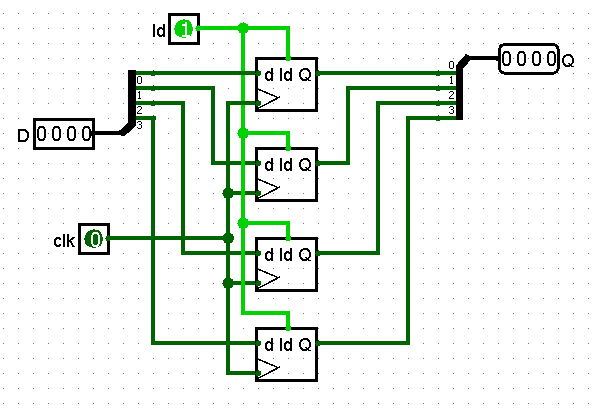
\includegraphics{q6-3-1.PNG}
\\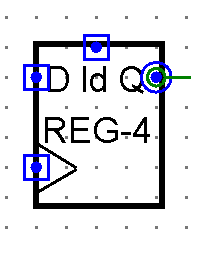
\includegraphics{q6-3-2.PNG}
\\
We are now ready to construct the Program Counter. It has the following specification:

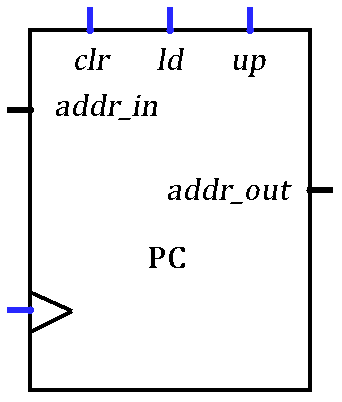
\includegraphics[height=3.5cm]{images/PC.png}

\begin{tabular}{c c c | l}
$clr$ & $ld$ & $up$ & function \\
\hline
0 & 0 & 0 & No change \\
0 & 0 & 1 & $PC \leftarrow PC + 1$ \\
0 & 1 & X & $PC \leftarrow addr\_in$ \\
1 & X & X & $PC \leftarrow 0$ \\
\end{tabular}

In the table above, $PC$ is understood to mean the state/contents of the PC register.

Suppose $addr\_in$, and the register contents $PC$ each have 4 bits. Then the characteristic table for this device would have $2^{11}=2048$ rows! Fortunately instead of creating a purpose-built device using the characteristic table, we can observe the overall functionality from the functional description given above instead of analyzing the behaviour of individual bits.

\item[6] In Logisim, using one (1) of your 4-bit parallel load registers you constructed, two (2) 4-bit $2 \times 1$ multiplexers, one (1) 4-bit full adder, and any logic gates and power/ground devices that you need, construct a circuit that satisfies the required behaviour of the program counter. Draw your circuit diagram here. To produce the necessary multiplexers in Logisim, set "Select Bits" to 1, "Data Bits" to 4, "Disabled Output" to Zero, "Include Enable?" to No.


\\
\\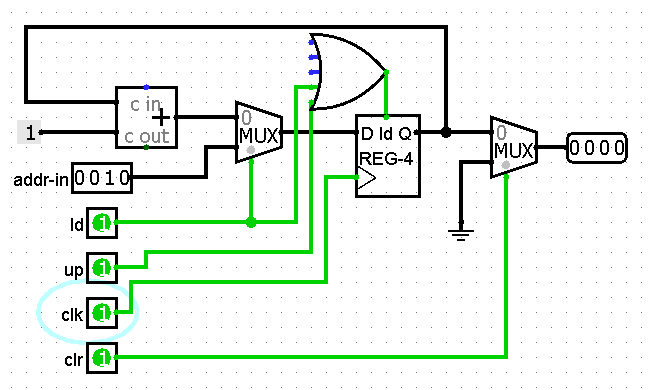
\includegraphics{q6-4-1.PNG}
\\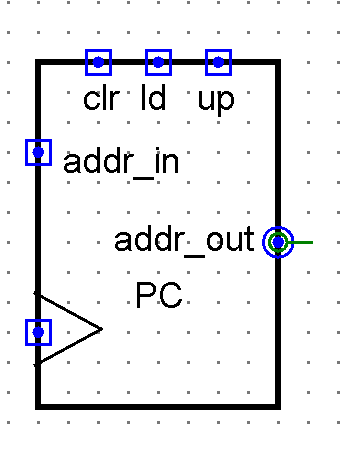
\includegraphics{q6-4-2.PNG}
\\
\end{question}

\newpage